\documentclass[11pt,a4paper,titlepage]{article}

% packages

\usepackage[spanish]{babel}
\usepackage[utf8]{inputenc}
\usepackage{amsmath}
\usepackage{amsfonts}
\usepackage{amssymb}
\usepackage{graphicx}
\usepackage{titling}
\usepackage{microtype}
\usepackage{listings}
\usepackage{xcolor}

\newsavebox\thmbox
\newtheorem{mytheorem}{}
\newenvironment{theorem}%
  {\begin{lrbox}{\thmbox}%
   \begin{minipage}{\dimexpr\linewidth-2\fboxsep}
   \begin{mytheorem}}%
  {\end{mytheorem}%
   \end{minipage}%
   \end{lrbox}%
   \begin{trivlist}
     \item[]\colorbox{lightgray}{\usebox\thmbox}
   \end{trivlist}}

% commands

\newcommand{\Cite}[1]{\textbf{[#1]}}
\newcommand{\Scalar}[1]{\ensuremath{\mathnormal{#1}}}
\newcommand{\Two}[1]{\ensuremath{\mathbf{#1}}}
\newcommand{\Three}[1]{\ensuremath{\mathbf{#1}}}
\newcommand{\Mat}[1]{\ensuremath{\mathbf{\hat{#1}}}}
\newcommand{\TwoCart}[1]{\ensuremath{\mathbf{\dot{#1}}}}
\newcommand{\ThreeCart}[1]{\ensuremath{\mathbf{\dot{#1}}}}
\newcommand{\Vector}[1]{\ensuremath{\left[#1\right]^T}}
\newcommand{\Axis}[1]{\ensuremath{\mathrm{#1}}}
\newcommand{\Plane}[1]{\ensuremath{\mathrm{#1}}}
\newcommand{\Figure}[1]{Figura #1}
\newcommand{\Section}[1]{#1}

% title page

\title{Estudio comparativo sobre visión estéreo en tiempo real para cámaras de recursos limitados}
\author{Darío Sneidermanis \\ Darío Susnisky}
\predate{\center}
\date{Noviembre 2015}
\postdate{\vfill
	\center{Proyecto final tutelado por Juan Miguel Santos}
	\center{Departamento de Ingeniería Informática}
	\center{Instituto Tecnológico de Buenos Aires}\\
}

% document

\begin{document}

\maketitle
\tableofcontents
\clearpage

% Set space between paragraphs to one line (has to be after the table of contents)
\setlength{\parskip}{\baselineskip}

\section{Resumen}

En los últimos 15 años ha habido un avance considerable en el campo de visión estéreo, específicamente en los algoritmos de tiempo real. La mejora y abaratamiento constante tanto de cámaras como de procesadores ha incentivado la investigación en este campo, logrando importantes avances. En este trabajo realizamos una comparación teórica y experimental de algoritmos pertenecientes al actual estado del arte para reconstrucción de información tridimensional a partir de cámaras estéreo. Para la comparación experimental se eligió una cámara de baja gama y fácil obtención en el mercado, llamada Minoru.

\newpage

\section{Introducción}

Si bien una imagen es un conjunto de puntos en dos dimensiones, nosotros vivimos en un mundo en tres dimensiones en donde las escenas tienen volumen y están espacialmente dispuestas de forma tal que los objetos pueden estar tapándose entre sí. Aunque para nosotros son datos intuitivos, el procesamiento de imágenes suele ser un desafío complejo que se ha venido estudiando por más de 50 años. La habilidad para utilizar los datos de la tercer dimensión juega un papel decisivo en el análisis de entornos estáticos o dinámicos. Un ejemplo evidente de uso de esta información es la mejora en la navegación de robots. En el campo médico, las nuevas tecnologías requieren información más precisa sobre profundidades. En general, el dominio del procesamiento 3D en fotografía digital, juegos por computadora, multimedia, visualización 3D y realidad aumentada pueden hacer un uso extensivo de datos 3D en tiempo real.

Dada la importancia y diversidad del uso de esta información, durante los últimos 15 años se han presentado nuevos algoritmos, y otros algoritmos existentes han sido mejorados con el propósito de obtener resultados más precisos de forma más veloz. La naturaleza del problema hace que tanto la precisión como la velocidad sean factores no triviales. La precisión de los resultados es afectada por información faltante en una imagen 2D (como oclusiones o superficies en donde las profundidades varían según el punto de vista del observador). Las dificultades de la calibración de las dos cámaras es una de las tantas razones por las cuales la obtención de resultados ideales sigue siendo un problema considerado sin resolver completamente. Además, la cantidad de píxeles en cada imagen aumenta la cantidad de cálculos requeridos, haciendo que el problema de la correspondencia sea uno computacionalmente complejo limitando severamente la velocidad con la que se pueden obtener resultados. En muchos casos, la velocidad y la precisión se enfrentan entre sí, haciendo que sea difícil mejorar ambos aspectos de forma simultánea, teniéndose que definir este balance en base a la aplicación concreta. Constantemente se pueden ver aplicaciones que podrían beneficiarse de los datos en la tercer dimensión. Este incremento en las posibles aplicaciones está inherentemente asociado a la facilidad de obtener sensores de imágenes básicos, económicos y de baja calidad, encontrados en teléfonos celulares, consolas, cámaras de seguridad y drones entre otros. Además de la baja resolución de las imágenes, estos dispositivos suelen tener recursos computacionalmente limitados haciendo que el desafío sea aún mayor.

Los esfuerzos en resolver este problema presentan en la actualidad un conjunto extenso de algoritmos disponibles para solucionar esta cuestión, exponiendo distintos balances entre precisión y velocidad. Si bien existen diversos trabajos que comparan estos algoritmos de forma extensa, pocas fuentes informan sobre la viabilidad de dichos algoritmos en sistemas de bajos recursos.

Este trabajo presenta un análisis y comparación de tres algoritmos evaluando precisión, tiempo, densidad y rango de los mismos en una cámara Minoru la cual es económica y de fácil obtención en el mercado. Además se expone un estudio sobre el uso de cámaras de este estilo y sus posibles aplicaciones.

Los algoritmos estudiados son \textit{Block Matching} (BM) \Cite{K98}, \textit{Semi Global Block Matching} (SGBM) \Cite{H05} \Cite{EH08} y \textit{Efficient Large-scale Stereo} (ELAS) \Cite{GRU11}. Para la implementación de los primeros dos algoritmos se utilizó la librería OpenCV, mientras que para ELAS se utilizó LibELAS, librería producida por los autores del algoritmo original. Todos los algoritmos traen como resultado un mapa de disparidad. Un mapa de disparidad refiere a la distancia aparente de píxeles entre un par de imágenes estéreo. Para experimentar esta distancia obtenida, uno puede cerrar cada uno de los ojos de forma desfasada. Al hacer esto, los objetos más cercanos parecen moverse una distancia más significativa que los objetos más alejados. Como resultado, un mapa de disparidad permite visualizar en base a intensidades de grises o gamas de colores la profundidad de la escena.

En el segundo capítulo se hará una explicación detallada del marco teórico necesario para poder comprender el funcionamiento de dichos algoritmos, presentando así una introducción a la geometría proyectiva para luego explicar el modelo de una cámara. Luego, en este capítulo se explican nociones sobre la visión estéreo incluyendo conceptos como calibración, rectificación y geometría epipolar. Para darle un cierre al marco teórico se profundiza sobre el concepto de mapa de disparidad. En el tercer capítulo se realizará una explicación detallada sobre cada uno de los algoritmos evaluados, explicando la forma en la que cada uno de estos obtiene un mapa de disparidad. En el cuarto capítulo se expone la experimentación realizada, presentando una comparación entre los distintos algoritmos. Finalmente, en el quinto capítulo se presentan las conclusiones del trabajo, evaluando tanto las comparaciones entre los algoritmos como la viabilidad de su uso en sistemas de bajos recursos. En este capítulo también se proponen aplicaciones y trabajos futuros.

\newpage

\section{Marco teórico}

\subsection{Geometría proyectiva}

La geometría euclidiana con la que estamos familiarizados describe muy bien nuestro mundo tridimensional: los lados de objetos tienen longitudes, las líneas que se intersectan forman ángulos entre sí, y dos líneas se dicen paralelas si están en el mismo plano y nunca se cruzan. Más aún, estas propiedades no cambian al aplicar transformaciones euclidianas (transformación y rotación).

Sin embargo, al considerar el proceso de captura de una imagen en una cámara, este modelo ya no es suficiente: las longitudes y ángulos no se preservan, y las líneas paralelas pueden llegar a cortarse. La geometría proyectiva, que es una generalización de la euclidiana, provee un marco mucho más versátil para expresar la geometría de una cámara, permitiendo una cantidad de transformaciones mucho más amplia.\footnote{En \Cite{CM03} se hace un desarrollo completo de esta geometría y sus propiedades.}

Las coordenadas utilizadas en geometría proyectiva son llamadas coordenadas homogéneas, o proyectivas, y se hace un uso extenso de ellas en este trabajo. Para ello se emplea la siguiente notación:

\begin{itemize}
	\item Los escalares son representados con letras en cursiva (ej. \Scalar{s}).
	\item Los vectores son representados con:
	\begin{itemize}
		\item letras minúsculas en negrita (ej. \Two{m}) si pertenecen a un espacio de 2 dimensiones (de ahora en más, 2D).
		\item letras mayúsculas en negrita (ej. \Three{M}) si pertenecen a un espacio de 3 dimensiones (de ahora en más, 3D).
	\end{itemize}
	\item Las matrices son representadas con letras mayúsculas en negrita, con un sombrero (ej. \Mat{A}).
\end{itemize}

\subsubsection{Punto}

Sea $\ThreeCart{M} = \Vector{\Scalar{x}, \Scalar{y}, \Scalar{z}}$ un punto en el espacio 3D expresado en coordenadas cartesianas, en el espacio proyectivo es representado como $\Three{M} = \Vector{\Scalar{x}, \Scalar{y}, \Scalar{z}, 1}$. En general, el punto $\Three{M} = \Vector{\Scalar{x}, \Scalar{y}, \Scalar{z}, \Scalar{t}}$ corresponde al punto $\ThreeCart{M} = \Vector{\Scalar{x}/\Scalar{t}, \Scalar{y}/\Scalar{t}, \Scalar{z}/\Scalar{t}}$. De la misma manera, \TwoCart{m} es representado como \Two{m}.

\subsubsection{Recta}

Una recta en el espacio 2D puede ser representada por un vector en el espacio 3D: el punto \TwoCart{m} pertenece a la recta \Two{l} (donde $\Two{l} = \Vector{\Scalar{a}, \Scalar{b}, \Scalar{c}}$) si y sólo si $\Two{l} \cdot \Two{m} = 0$. En el plano proyectivo la representación de una recta es igual a la representación de un punto (principio de dualidad).

\subsubsection{Plano}

Un plano en el espacio 3D puede ser representado por un vector en el espacio 4D: un punto \ThreeCart{M} pertenece al plano \Plane{\Pi} (donde $\Plane{\Pi} = \Vector{\Scalar{a}, \Scalar{b}, \Scalar{c}, \Scalar{d}}$) si y sólo si $\Plane{\Pi} \cdot \Three{M} = 0$.

\subsection{Modelo de una cámara}

Para estudiar la matemática de un sistema de cámaras estéreo empezamos modelando una única cámara ideal, también conocida como cámara estenopeica. En la \Figure{1} se muestra una cámara ideal con centro óptico en el origen del sistema de coordenadas del mundo $\left( \Axis{X_m}, \Axis{Y_m}, \Axis{Z_m} \right)$, y longitud focal $\Scalar{f} = 1$. La recta que pasa por el centro óptico y el punto \ThreeCart{M} del mundo, corta al plano retinal \Plane{\Pi} en el punto \TwoCart{m} del sistema de coordenadas de la cámara $\left( \Axis{X_c}, \Axis{Y_c} \right)$.

%%%%%%%%%
% Insert figure 1
%%%%%%%%%

\begin{figure}[h!]

  \centering
    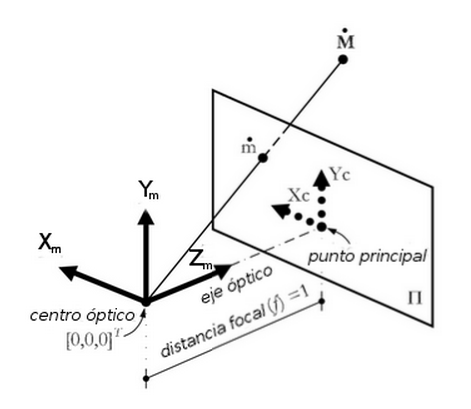
\includegraphics[width=0.6\textwidth]{f1.png}
  \caption{Modelo de cámara ideal.}
\end{figure}

\subsubsection{Matriz de la cámara}

La principal propiedad del modelo de la cámara es que los puntos (pixels) en el plano retinal (imagen) son una proyección lineal de los puntos en el mundo:
\[
	\Two{m} \simeq \Mat{P}\Three{M}
\]
donde \Mat{P} es una matriz de $3 \times 4$ llamada matriz de la cámara, y el signo $\simeq$ significa que los lados de la ecuación difieren únicamente por un factor escalar.

Como el origen del sistema de coordenadas del mundo coincide con el centro óptico de la cámara, y la distancia focal es $1$, \Mat{P} es igual a $\Mat{P_c}$, la matriz de una cámara ideal:
\[
	\Mat{P} = \Mat{P_c} =
	\begin{bmatrix}
		1 & 0 & 0 & 0 \\
		0 & 1 & 0 & 0 \\
		0 & 0 & 1 & 0
	\end{bmatrix}
\]

\subsubsection{Parámetros intrínsecos y extrínsecos}

En la \Figure{2} se puede observar el caso general, en el cual los orígenes de coordenadas del mundo y de la cámara pueden estar localizados arbitrariamente en el espacio, y la longitud focal no necesariamente vale $1$.

%%%%%%%%%
% Insert figure 2
%%%%%%%%%

\begin{figure}[h!]

  \centering
    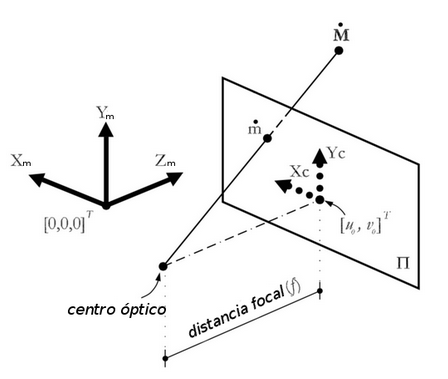
\includegraphics[width=0.6\textwidth]{f2.png}
  \caption{Modelo de una cámara (caso generalizado).}
\end{figure}

Hacer un cambio de coordenadas en el plano retinal equivale a multiplicar \Mat{P} por izquierda por una matriz \Mat{A} de $3 \times 3$, y un cambio de coordenadas en el espacio del mundo equivale a multiplicar \Mat{P} por derecha por una matriz \Mat{D} de $4 \times 4$:
\[
	\Mat{P} = \Mat{A}\Mat{P_c}\Mat{D}
\]
donde
\begin{itemize}
	\item \Mat{A} es la matriz de calibración de la cámara, que transforma las coordenadas de la imagen normalizada a las coordenadas de la imagen retinal. Se dice que una cámara está calibrada cuando se conoce \Mat{A}. Los parámetros de esta matriz son llamados parámetros intrínsecos de la cámara por ser independientes de la escena:
	\[
		\Mat{A} =
		\begin{bmatrix}
			\Scalar{f} \Scalar{k_u} & 0 & \Scalar{u_0} \\
			0 & \Scalar{f} \Scalar{k_v} & \Scalar{v_0} \\
			0 & 0 & 1
		\end{bmatrix}
	\]
	con
	\begin{itemize}
		\item \Scalar{f} es la longitud focal de la cámara.
		\item \Scalar{k_u} y \Scalar{k_v} son los factores de escala horizontal y vertical respectivamente.
		\item \Scalar{u_0} y \Scalar{v_0} son las coordenadas del punto principal de la cámara (ver \Figure{1} y \Figure{2}).
	\end{itemize}
	\item \Mat{D} es la matriz que describe el cambio de pose de la cámara en el sistema de coordenadas del mundo. Los parámetros de esta matriz son llamados parámetros extrínsecos de la cámara:
	\[
		\Mat{D} =
		\begin{bmatrix}
			\Mat{R} & \ThreeCart{T} \\
			\mathbf{0}^T_3 & 1
		\end{bmatrix}
	\]
	con
	\begin{itemize}
		\item \Mat{R} es una matriz de rotación de $3 \times 3$.
		\item \ThreeCart{T} es un vector 3D de traslación.
	\end{itemize}
\end{itemize}

Para un análisis más profundo del modelo de una cámara ideal y sus propiedades, referirse a \Cite{EL03}.

\subsubsection{Coeficientes de distorción}

Al usar cámaras reales, especialmente si son de baja gama, las imperfecciones en las lentes pueden distorsionar las imágenes capturadas. En general esto no es un problema, ya que las distorsiones pueden ser corregidas por software directamente sobre las capturas. Los tipos de distorsión más comunes son la radial y la tangencial.

La distorsión radial hace que líneas rectas en el espacio aparezcan curvas en la imagen. Este efecto es causado por imperfecciones radialmente simétricas de la lente fotográfica. Por ejemplo, en la \Figure{3} se han unido con líneas rectas rojas cuatro vértices del tablero, dejando en evidencia que los bordes no son rectos.

%%%%%%%%%
% Insert figure 3
%%%%%%%%%

\begin{figure}[h!]

  \centering
    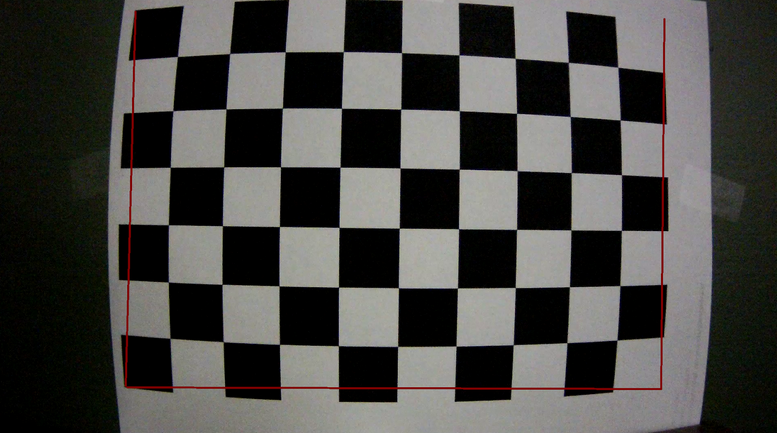
\includegraphics[width=1\textwidth]{f3.png}
  \caption{Fotografía con distorsión radial de un tablero de ajedrez.}
\end{figure}

Esta distorsión se puede corregir usando el modelo de Brown–Conrady (ver \Cite{B66}):
\begin{align*}
	x_\mathrm{corregido} &= x \left( 1 + k_1 r^2 + k_2 r^4 + k_3 r^6 \right) \\
	y_\mathrm{corregido} &= y \left( 1 + k_1 r^2 + k_2 r^4 + k_3 r^6 \right)
\end{align*}
con $r^2 = x^2 + y^2$.

Este modelo también permite corregir las distorsiones tangenciales, causadas cuando la lente no está perfectamente paralela con el plano de la imagen:
\begin{align*}
	x_\mathrm{corregido} &= x + \left[ 2 p_1 x y + p_2 \left( r^2 + 2x^2 \right) \right] \\
	y_\mathrm{corregido} &= y + \left[ 2 p_2 x y + p_1 \left( r^2 + 2y^2 \right) \right]
\end{align*}
con $r^2 = x^2 + y^2$.

Los coeficientes de estas transformaciones son llamados coeficientes de distorsión. Al ser independientes de la escena, son también parámetros intrínsecos de la cámara.
\[
	\textrm{coeficientes\ de\ distorsi\'on} = \left( k_1,\  k_2,\  p_1,\  p_2,\  k_3 \right)
\]

\subsection{Calibración}

Dado que los parámetros intrínsecos de una cámara no cambian con la escena, se pueden precalcular para simplificar los análisis posteriores. Este proceso es llamado calibración.

La calibración puede realizarse de varias maneras\footnote{En \Cite{Z04} se realiza un excelente desarrollo y comparación de las distintas técnicas de calibración.}, siendo la más común por su simpleza y precisión la calibración con un patrón 2D. Este método consiste en capturar un mismo patrón bidimensional en diferentes orientaciones, y resolver las ecuaciones geométricas asociadas.

En particular, se realizan varias (más de 10) capturas de un patrón tipo tablero de ajedrez como el de la \Figure{3}, en diferentes poses. Se elige un tablero de ajedrez por tener características fácilmente reconocibles, como las esquinas de los cuadrados. Cada una de estas capturas añade una nueva ecuación relacionando las coordenadas 3D de puntos del patrón en la escena, con puntos 2D en la imagen. Finalmente, estas ecuaciones pueden ser resueltas usando un algoritmo de aproximación, como el de \Cite{Z00}, para obtener los parámetros de la cámara.

\noindent
El proceso de calibración puede resumirse en los siguientes pasos:
\begin{enumerate}
	\item Imprimir un patrón y pegarlo a una superficie plana.
	\item Tomar varias capturas del patrón en distintas orientaciones.
	\item Detectar puntos característicos en las imágenes capturadas.
	\item Estimar los parámetros intrínsecos y extrínsecos como si las lentes no tuvieran distorsiones.
	\item Estimar los coeficientes de distorsión usando el método de cuadrados mínimos.
	\item Refinar los parámetros utilizando el método de estimación por máxima verosimilitud.
\end{enumerate}

Es posible calcular un error de reproyección, que indica cuán buenos son los parámetros obtenidos. Este error se calcula tomando la media, para todas las capturas, de las distancias entre los puntos característicos en la imagen capturada, y en la imagen proyectada con los parámetros obtenidos.

\subsection{Visión estéreo}

Se llama análisis estéreo al proceso de medir la distancia a un objeto a partir de la comparación de las proyecciones del objeto en dos o más imágenes. El problema fundamental en el análisis estéreo es encontrar elementos correspondientes entre las imágenes. Una vez que se encuentra una correspondencia, la distancia del objeto a las cámaras puede ser calculada a partir de la geometría de las imágenes.

Para nuestras cámaras estéreo la traslación \ThreeCart{T} y orientación \Mat{R} relativa entre las dos cámaras es fija. Es decir, dada la matriz de rotación y traslación de la primer cámara (\Mat{R_1} y \ThreeCart{T_1}) es posible calcular la pose de la segunda cámara (\Mat{R_2} y \ThreeCart{T_2}) mediante:
\begin{align*}
	\Mat{R_2} &= \Mat{R} \, \Mat{R_1} \\
	\ThreeCart{T_2} &= \Mat{R} \, \ThreeCart{T_1} + \ThreeCart{T}
\end{align*}

De forma opcional se puede calcular la matriz esencial \Mat{E}:
\[
	\Mat{E} =
	\begin{bmatrix}
		0 & -\ThreeCart{T}(3) & \ \ \ThreeCart{T}(2) \\
		\ \ \ThreeCart{T}(3) & 0 & -\ThreeCart{T}(1) \\
		-\ThreeCart{T}(2) & \ThreeCart{T}(1) & 0
	\end{bmatrix}
	\times \Mat{R}
\]

Si \TwoCart{m} y  \TwoCart{m'} son las proyecciones sobre los planos retinales de cada cámara correspondientes a un punto tridimensional \ThreeCart{M} en cada imagen, se cumple que:
\[
	\Two{m'}^T \Mat{E} \Two{m} = 0
\]

\subsubsection{Geometría epipolar}

La geometría epipolar es aquella que surge al analizar el problema de correspondencia de puntos en imágenes estéreo. Es de particular interés la curva epipolar, ilustrada en la \Figure{4}.

Tomando un punto \TwoCart{m} en la imagen \Plane{I_1}, consideramos la recta que parte del centro óptico \ThreeCart{C_1}, y corta \Plane{I_1} en \TwoCart{m}, que intersecta objetos en la escena a diferentes distancias. La proyección de esta recta en la \Plane{I_2} es la curva epipolar asociada a \TwoCart{m}. La importancia de esta curva parte del hecho que para cualquier objeto observado en el punto \TwoCart{m}, el punto correspondiente en la segunda imagen tiene que estar en la curva epipolar. Por lo tanto, alcanza con buscar sólo sobre esta línea al realizar la correspondencia de puntos.

%%%%%%%%%
% Insert figure 4
%%%%%%%%%

\begin{figure}[h!]

  \centering
    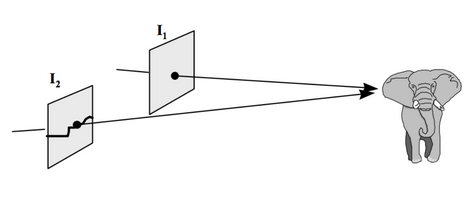
\includegraphics[width=0.6\textwidth]{f4.png}
  \caption{Ilustración de la curva epipolar. \Cite{K98}}
\end{figure}

Para el caso de cámaras estereoscópicas, una vez corregidas las distorsiones explicadas en la sección \Section{2.2.3}, las curvas epipolares son proyecciones de rectas en un plano, y por lo tanto líneas rectas. Para realizar la búsqueda de puntos correspondientes de manera eficiente, se realiza una transformación en las imágenes captadas, de tal manera que todas las líneas epipolares queden paralelas y horizontales. Este proceso es llamado rectificación, y se explica en la sección siguiente.

Supongamos que ambas cámaras observan un punto \ThreeCart{M}. Como se puede observar en la \Figure{5}, en la proyección de la cámara izquierda podemos definirlo como \ThreeCart{M_1} y en la cámara derecha como \ThreeCart{M_2}. A su vez, las cámaras tienen centros de proyección definidos como \ThreeCart{C_1}  y \ThreeCart{C_2}. Luego podemos proyectar cada centro de proyección hasta el plano de imagen de la otra cámara. El punto de intersección se denomina \textbf{punto epipolar} que notaremos como \TwoCart{e_1} y \TwoCart{e_2}.

Si bien el segmento que une a los puntos \ThreeCart{C_1} y \ThreeCart{M} es visto por la cámara izquierda como un punto, la cámara derecha lo puede ver como una línea. Esa línea proyectada en la vista de la cámara derecha (formada por el segmento $\overline{\TwoCart{e_2}\TwoCart{m_2}}$) es definido como una \textbf{línea epipolar}. Es así que una línea epipolar se define como una función del punto 3D \ThreeCart{M}. De esta manera, una línea epipolar siempre intersecta un punto epipolar y de hecho cualquier línea que cumpla esta condición se define como línea epipolar.

%%%%%%%%%
% Insert figure 5
%%%%%%%%%

\begin{figure}[h!]

  \centering
    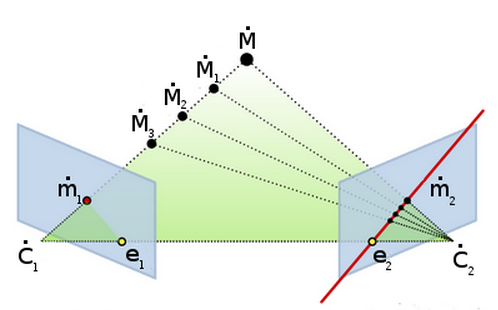
\includegraphics[width=0.8\textwidth]{f5.png}
  \caption{Líneas epipolares en visión estéreo.}
\end{figure}

A su vez, como visualización alternativa, podemos definir al plano que une a los puntos \ThreeCart{M}, \ThreeCart{C_1} y \ThreeCart{C_2} como plano epipolar que intersecta a los planos de ambas imágenes.

\subsubsection{Rectificación}

La rectificación de las imágenes es un proceso de transformación de las mismas que permite proyectar dos (o más) imágenes en un plano en común. Esto se utilizará para simplificar el problema de encontrar puntos correspondientes entre ambas imágenes. Para explicar el proceso de rectificación, es importante comprender la geometría epipolar que describen las cámaras.

Dado que los puntos \ThreeCart{C_1} y \ThreeCart{C_2} son conocidos, si contamos también con los puntos \ThreeCart{M_1} y \ThreeCart{M_2} entonces podemos conocer la línea epipolar que intersecta a \TwoCart{e_1} y \TwoCart{e_2}. A partir de esto se puede deducir un conjunto de restricciones que permiten saber si dos puntos (de ambas cámaras) representan el mismo punto 3D en el mundo real. A su vez, estas restricciones pueden resumirse en lo que se conoce como la \textbf{matriz esencial} y la \textbf{matriz fundamental} entre las cámaras.

Para rectificar ambas imágenes buscamos que los puntos epipolares se muevan al infinito. En esa instancia, las líneas epipolares entre las imágenes se vuelven paralelas.

La \Figure{6} ilustra el proceso de rectificación.

%%%%%%%%%
% Insert figure 6
%%%%%%%%%

\begin{figure}[h!]

  \centering
    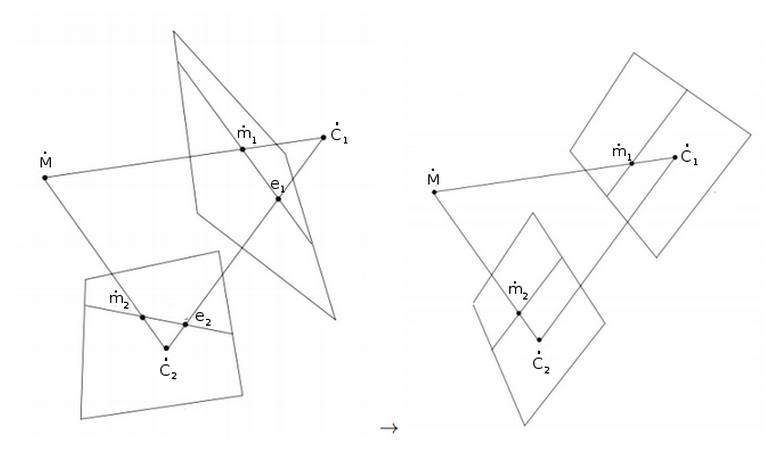
\includegraphics[width=1\textwidth]{f6.png}
  \caption{Ilustración del proceso de rectificación.}
\end{figure}

Para llevar a cabo la rectificación se debe proceder como se describe a continuación.

En primer lugar, se da por sentado que se cuenta con la matriz interna de ambas cámaras (\Mat{A_1} y \Mat{A_2}), sus matrices de rotación (\Mat{R_1} y \Mat{R_2}) y sus vectores de traslación (\ThreeCart{T_1} y \ThreeCart{T_2}). Estos datos han sido obtenidos en la fase de calibración. Así, podemos construir la matriz de proyección de la siguiente manera (donde $n$ puede hacer referencia a cualquiera de las cámaras):
\[
	\Mat{P_n} = \Mat{A_n} \left[ \Mat{R_n} | \ThreeCart{T_n} \right]
\]

En segundo lugar, se construye una nueva matriz rotacional \Mat{R'} (única para ambas cámaras). Esta matriz se construye asegurando que en el nuevo sistema de referencia de las cámaras el eje horizontal sea paralelo a la línea que se forma entre ambos centros ópticos.

En tercer lugar, se construye una nueva matriz interna \Mat{A'} (única para ambas cámaras). Existen diversas maneras para una construcción efectiva de esta matriz. En este caso se construyó en base a la media calculada entre ambas matrices internas originales (\Mat{A_1} y \Mat{A_2}).

En cuarto lugar, podemos construir una nueva matriz de proyección para cada cámara. La forma de obtención de dicha matriz se presenta a continuación donde $n$ puede hacer referencia una vez más a la cámara de la izquierda o a la cámara de la derecha:
\[
	\Mat{P'_n} = \Mat{A'} \left[ \Mat{R'} | -\Mat{R'} \ThreeCart{C_n} \right]
\]

Por último, se genera una correspondencia entre los planos de las imágenes originales a las nuevas matrices de proyección.

\subsection{Reconstrucción 3D}

Para reconstruir una escena 3D a partir de un par de imágenes capturadas con una cámara estéreo, se calcula una nube de puntos en el espacio tridimensional. Esta nube es representada mediante un mapa de disparidad.

\subsubsection{Triangulación}

Como se ilustra en la \Figure{7}, un punto 3D \ThreeCart{M} se puede calcular como la intersección de dos rectas pasando por los centros ópticos (\ThreeCart{C_1} y \ThreeCart{C_2}), y sus correspondientes proyecciones en las imagenes capturadas (\TwoCart{m_1} y \TwoCart{m_2}). Dado que estas dos rectas pertenecen a un mismo plano (plano epipolar), y los tres puntos \TwoCart{m_1}, \TwoCart{m_2} y \ThreeCart{M} forman un triángulo, este proceso se conoce como triangulación.

%%%%%%%%%
% Insert figure 7
%%%%%%%%%

\begin{figure}[h!]

  \centering
    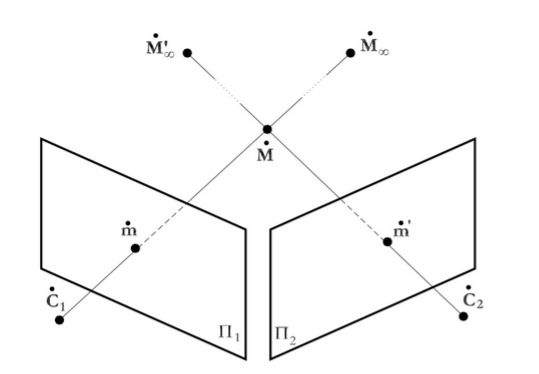
\includegraphics[width=0.7\textwidth]{f7.png}
  \caption{Ilustración del proceso de triangulación.}
\end{figure}

Sean \TwoCart{c_{1e}}, \TwoCart{c_{2e}}, \TwoCart{m_{1e}}, \TwoCart{m_{2e}} y \TwoCart{m_e} las representaciones de  \ThreeCart{C_1}, \ThreeCart{C_2}, \TwoCart{m_1}, \TwoCart{m_2}, y \ThreeCart{M}, respectivamente, en el sistema de coordenadas del plano epipolar, tenemos que:
\[
	\Two{m_e} = (\Two{c_{1e}} \times \Two{m_{1e}}) \times (\Two{c_{2e}} \times \Two{m_{2e}})
\]

Lamentablemente, debido a que en la realidad los parámetros y coordenadas son aproximados, las lentes imperfectas, y hay ruido en las imágenes, en general las rectas $<\ThreeCart{C_1}, \TwoCart{m_1}>$ y $<\ThreeCart{C_2}, \TwoCart{m_2}>$ no se cortan en un punto. En estos casos la triangulación se plantea como un problema de minimización para encontrar el punto que mejor aproxima la intersección. En \Cite{HS97} se puede ver un análisis del problema y comparación de varios métodos para resolverlo.

\subsubsection{Mapa de disparidad}

El mapa de disparidad, o mapa de profundidad, almacena una nube de puntos en el espacio 3D correspondientes a los pixels de una imagen. El mapa es un vector bidimensional en donde en cada posición $(\Scalar{x}, \Scalar{y})$ se guarda la distancia de ese punto 3D (\Scalar{z}) al plano retinal. Este mapa puede ser interpretado como una imagen de escala de grises, en donde la intensidad de cada pixel corresponde al valor de profundidad de ese pixel.

Para generar este mapa se hace una correspondencia entre los pixels de las dos imágenes estéreo. Midiendo la distancia entre cada par de puntos $\Scalar{x} - \Scalar{x'}$, mediante el proceso de triangulación se puede calcular la distancia \Scalar{z} al plano retinal.

El mapa de disparidad generado será utilizado para reconstruir la escena. A continuación se presentan varios algoritmos para realizar la correspondencia entre pixels.

\subsection{Cálculo de profundidad}

Dado el valor de disparidad de un punto, se puede calcular su profundidad, o distancia al centro de la cámara.

\begin{figure}[h!]
  \centering
    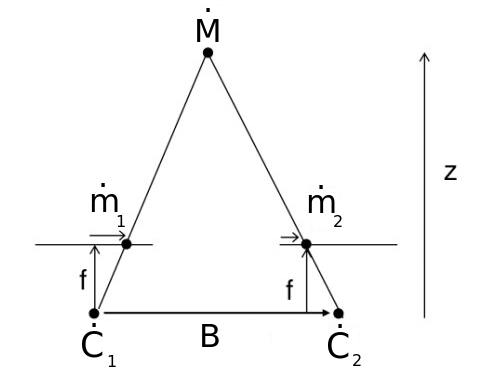
\includegraphics[width=0.7\textwidth]{fnew.png} %% CHANGE FIGURE
  \caption{Ilustración del proceso de triangulación.}
\end{figure}

En el diagrama anterior, queremos calcular la profundidad (\Scalar{z}) a partir la disparidad, es decir, la distancia entre los puntos en el plano de la imagen, correspondiendo al punto 3D \Three{X} de la escena:

\[
    disparidad = B - (x - x')
\]

donde \Scalar{B} es la apertura horizontal de la cámara estéreo (distancia entre los centros de las dos cámaras).

Dado que los triángulos $Xxx'$ y $XOO'$ son semejantes, podemos plantear:

\begin{align*}
    \frac{x - x'}{B} & = \frac{z - f}{z} \\
    x - x' & = B - \frac{Bf}{z} \\
    B - (x - x') & = \frac{Bf}{z} \\
    disparidad & = \frac{Bf}{z} \\
    z & = \frac{Bf}{disparidad}
\end{align*}

donde $f$ es la distancia focal de las cámaras.

\newpage

\section{Métodos de obtención de correspondencias}

Los métodos de obtención de correspondencias pueden ser categorizados entre \textit{locales} y \textit{globales}. Los métodos locales intentan encontrar correspondencias entre pequeñas regiones de una imágen y otra, a partir de características intrínsecas a la región. Los métodos globales suplementan a los locales considerando propiedades físicas, como continuidad de superficies.

Los métodos locales pueden ser subclasificados según busquen correspondencias entre \textit{características} discretas, o entre pequeñas \textit{áreas} de la imagen. Las características elegidas suelen ser independientes de la iluminación y del punto de vista, como por ejemplo esquinas de objetos. Los algoritmos basados en características funcionan especialmente bien cuando hay grandes diferencias entre los puntos de vista de las cámaras, o distintos tipos de cámaras, encontrando correspondencias de manera rápida y robusta. Sin embargo, tienen la desventaja de requerir una etapa previa de extracción de características potencialmente compleja, y los resultados (pares de puntos correspondientes) son poco densos.

Los métodos basados en área comparan pequeñas secciones de las imágenes. Hay una relación de compromiso con el área de estas secciones: áreas más chicas tienen más chances de ser detectadas en ambas imágenes, y áreas más grandes incrementan la proporción señal/ruido. A diferencia de los métodos basados en características, estos métodos producen resultados densos. Dado que no necesitan extraer características y que suelen tener estructuras algorítmicas muy regulares (ej. convoluciones), pueden implementarse de manera eficiente.

A continuación se presentan tres algoritmos de obtención de correspondencias.

\subsection{Block Matching}

Konolige \Cite{K98} propone un algoritmo que permite la obtención de un mapa de disparidad a través del análisis de bloques dentro de las imágenes. Con el tiempo, BM (Block Matching) se ha vuelto el enfoque más común e intuitivo para el cálculo de disparidades. La idea de un algoritmo que se basa en el análisis de áreas de la imagen consiste en deslizar un bloque tomado de una imagen sobre la segunda. Por cada movimiento del bloque se calcula un error. Originalmente, este algoritmo surge de la necesidad de calcular diferencias de movimiento entre dos imágenes. Dado el error encontrado en la correspondencia de bloques, se pueden encontrar la disparidad de los puntos en los bloques.

Puntualmente el algoritmo propuesto por Konolige busca una correlación en los bloques tras aplicar la transformada LOG (transformada del laplaciano sobre el gaussiano) con norma L1. Konolige decide el uso de esta transformada con esta norma dado que obtiene resultados de buena calidad que son optimizables dado el conjunto de instrucciones disponibles en el hardware utilizado por el autor en el momento de desarrollo. Los cálculos de disparidad se realizan en áreas de 16, 24 o 32 píxeles. Por último, el algoritmo aplica dos funciones para filtrar los resultados. El primer operador aplicado para filtrar los resultados mide las texturas en dirección a las líneas epipolares. Este operador es el propuesto por Matthies \Cite{M93}. Si bien este operador requiere una cota, la obtención de este valor se vuelve sencilla basándose en el ruido presentado en las imágenes de entrada. Tras aplicar el operador de Matthies, siguen presentándose errores causados por bloques correlativos solapados en áreas con disparidades muy distintas. Para eliminar estos errores se aplica un operador de izquierda/derecha \Cite{BW93}. En los resultados provistos por Konolige, la combinación de ambos operadores demuestra ser efectiva al eliminar falsos positivos teniendo en cuenta el rendimiento del algoritmo.

Cabe destacar que el algoritmo presentado con Konolige toma consideraciones extra para la calibración de las cámaras lo cual queda desestimado teniendo en cuenta los métodos de calibración y rectificación actuales ya presentados en este trabajo.

\subsection{Semi Global Block Matching}

El método SGBM (Semi Global Block Matching), presentado en \Cite{H05}, y posteriormente refinado en \Cite{H08}, es un método global de correspondencia entre píxeles que permite la obtención de un mapa de disparidad. La esencia de este algoritmo es calcular el mínimo de una función de evaluación de energía, utilizando un algoritmo de optimización con programación dinámica.

Scharstein y Szeliski \Cite{SS02} distinguen cuatro pasos que suelen realizarse en métodos para realizar la correspondencia entre píxeles. Estos cuatro pasos son:
\begin{itemize}
	\item Cálculo del costo de correspondencia
	\item Suma de los costos
	\item Cálculo de la disparidad
	\item Refinación de la disparidad
\end{itemize}

SGBM toma este modelo realizando implementaciones novedosas sobre cada uno de estos pasos.

\subsubsection{Cálculo del costo de correspondencia}

El costo de correspondencia, que forma la base de los algoritmos de búsqueda de correspondencias, se refiere al costo de correspondencia de pixels entre dos o más imágenes. SGBM elige usar la función de costo presentada en \Cite{BT98}, que utiliza una interpolación a nivel de los sub-píxeles.

Dado $\phi_L(x, y)$ y $\phi_R(x, y)$, la intensidad del pixel en la posición $(x, y)$ para las cámaras izquierda y derecha, y la distancia de separación \Scalar{d}, definimos la intensidad mínima y máxima como:
\begin{align*}
	\phi_R^- &= \frac{1}{2} \left( \phi_R( x + d, y ) + \phi_R( x + d - 1, y ) \right ) \\
	\phi_R^+ &= \frac{1}{2} \left( \phi_R( x + d, y ) + \phi_R( x + d + 1, y ) \right )
\end{align*}
\begin{align*}
	\phi_\mathrm{min} &= \mathrm{min} \left( \phi_R^-,\ \phi_R( x + d, y ),\ \phi_R^+ \right ) \\
	\phi_\mathrm{max} &= \mathrm{max} \left( \phi_R^-,\ \phi_R( x + d, y ),\ \phi_R^+ \right )
\end{align*}

Y con estas fórmulas se define la función de costo de correspondencia en un punto $(x, y)$ con una separación \Scalar{d} como:
\[
	F(x, y, d) = \mathrm{max} \left\{ 0,\ \phi_L(x, y) - \phi_\mathrm{max},\ \phi_\mathrm{min} - \phi_L(x, y) \right\}
\]

Esta función tiene en cuenta las intensidades de otros puntos en el área, para ser menos sensible al ruido.

\subsubsection{Suma de los costos}

La suma de los costos implica conectar los costos de correspondencia dentro de un vecindario de píxeles cercanos. Se suele sumar dentro de una ventana fija a disparidad constante. SGBM define el costo teniendo en cuenta el contexto de un pixel como:
\begin{align*}
	L_\Delta(x, y, d) = F(x, y, d) + \mathrm{min} & [ \\
	                                                              &\ L_\Delta(x - \Delta_x, y - \Delta_y, d), \\
	                                                              &\ L_\Delta(x - \Delta_x, y - \Delta_y, d - 1) + P_1,\\
	                                                              &\ L_\Delta(x - \Delta_x, y - \Delta_y, d + 1) + P_1,\\
	                                                              &\ \underset{i}{\mathrm{min}}\ L_\Delta(x - \Delta_x, y - \Delta_y, i) + P_2\\
	                                                              & ] - \underset{k}{\mathrm{min}}\ L_\Delta(x - \Delta_x, y - \Delta_y, k)
\end{align*}

donde $\Delta$ es una dirección, que puede recorrer los pixels adyacentes con 8-conectividad. Por lo tanto, la fórmula de costo de correspondencia total es:
\[
	C(x, y, d) = \sum_\Delta L_\Delta(x, y, d)
\]

\subsubsection{Cálculo de la disparidad}

Al obtener los costos de correspondencia de pixels, el cálculo de disparidad es relativamente simple. Para un píxel $(x, y)$ en la imagen izquierda la disparidad es:
\[
	d(x, y) = \underset{d}{\mathrm{min}}\ C\left( x, y, d \right)
\]

\subsection{Efficient Large-scale Stereo Matching}

ELAS (\textit{Efficient Large-scale Stereo}) propone un modelo generativo probabilístico para la correspondencia stereo entre píxeles mediante pequeñas ventanas de agregación reduciendo ambigüedades entre las correspondencias permitiendo la generación de un mapa de disparidad.

El enfoque propuesto por ELAS realiza un análisis preliminar en el espacio de disparidades al formar una triangulación basada en correspondencias robustas llamadas “puntos soporte”. Estos puntos contienen información valiosa a la hora de comparar el resto de los puntos de las imágenes. Las características principales que permiten identificar estos puntos son la textura y la unicidad. Para la obtención de los puntos soporte se utiliza una cuadrícula de 9x9 usando la distancia $l_1$ entre los vectores que se forman al concatenar filtros de Sobel horizontales y verticales. Las máscaras de Sobel tienen un tamaño de 3x3 y un paso de 5 píxeles.

Para asegurar que estos puntos son robustos, se asegura la consistencia haciendo la correspondencia de izquierda a derecha y de derecha a izquierda y solamente se consideran como válidos aquellos puntos que se destaquen al aplicar el filtro en todas las direcciones. Además se fija una cota para filtrar resultados precisos. En el caso de que algún punto correspondiente presente resultados poco similares a la mayoría se lo elimina considerándolo un caso espurio. Para asegurar que el algoritmo cubra la imagen de forma completa, se agregan puntos correspondientes en las cuatro esquinas cuyas disparidades se toman de los vecinos más cercanos.

ELAS propone un modelo generativo de la información. Para esto define el conjunto de puntos soporte como $S = \left\{ s_1, s_2, ... , s_m \right\}$. A su vez, $s_m = \left\{ u_m, v_m, d_m \right\}$, donde $u$ y $v$ son las coordenadas en el espacio y $d$ es la disparidad.

Dados los puntos soporte podemos definir al resto de los puntos de la imagen como “puntos observables” $O = \left\{ o_1, o_2, ... , o_m \right\}$. $o_m = \left\{ u_m, v_m, f_m \right\}$ donde $f$ es un vector de características distintivas (como por ejemplo, la intensidad del píxel). Al utilizar las letras $(l)$ y $(r)$ sobreescritas sobre un carácter indicaremos que se toma la imágen izquierda o derecha respectivamente.

Dado $S$ y un punto $o_n^{(l)}$ se calcula una disparidad $d_n$ mediante la probabilidad de una combinación entre una distribución uniforme y una Gaussiana:
%%%%%%%%%
% Insert equation
%%%%%%%%%

\[
	p(d_{n}|S,o_{n}^{(l)})\alpha
	\begin{cases}
	  \gamma + \text{exp} [ - (d_{n} - \mu(S,o_{n}^{(l)})^{2}) / 2 \sigma^{2} ] & \text{si } |d_{n} - \mu| < 3\sigma \vee d_{n} \in N_{S} \\
	  0 & \text{en cualquier otro caso}.
	\end{cases}
\]


Contando con estos datos podemos expresar la probabilidad de correspondencia con un punto $o_n^{(r)}$ con una distribución Laplaciana de la siguiente manera:
%%%%%%%%%
% Insert equation
%%%%%%%%%

\[
	p(o_{n}^{(r)}|o_{n}^{(l)},d_{n})\alpha
	\begin{cases}
	  \text{exp} ( - \beta || f_{n}^{(l)} - f_{n}^{(r)} ||_{1}) & \text{si } \binom{u_{n}^{(l)}}{v_{n}^{(l)}} = \binom{u_{n}^{(r)} + d_{n}}{v_{n}^{(r)}}\\
	  0 & \text{en cualquier otro caso}.
	\end{cases}
\]

Una vez definidos los puntos correspondientes basta con calcular la disparidad entre estos puntos para la generación del mapa de disparidad. Para este cálculo se utiliza una estimación \textbf{máximo a-posteriori} (MAP).

\newpage

\section{Comparación entre los algoritmos}

Este capítulo tiene como propósito comparar experimentalmente los tres métodos de obtención de un mapa de disparidad. Para esto se definen los indicadores a medir y el conjunto de experimentos a realizar. Además, se discute en detalle la implementación realizada y los entornos sobre los cuales se realizaron las pruebas.

\subsection{Indicadores}

No todos los métodos son igual de efectivos en las mismas escenas, ni todas las cámaras funcionan igual de bien en distintos escenarios. Por lo tanto, se toman en cuenta distintos indicadores para poder evaluar las fortalezas y debilidades de cada método en general, y de la cámara utilizada en particular.

\subsubsection{Precisión}

En los experimentos realizados se presentan objetos a distancias conocidas. Comparando estas distancias con las distancias calculadas por un método, se puede calcular la media del error como:

\[
	error=\frac{1}{\#capturas}\sum_{captura}\left|d_{conocida}-d_{calculada}\right|
\]

\subsubsection{Densidad}

Para determinar la densidad de información de profundidad media de cada método, se mide la densidad de píxeles con información de profundidad por captura.

\[
	densidad = \frac{1}{\#capturas} \sum_{captura} {\frac{\#pixeles\ con\ informacion}{\#pixeles\ por\ captura}}
\]

\subsubsection{Rango}

Se llama rango de la cámara al intervalo de distancia frente a esta en el cual, si se coloca un objeto, se puede calcular de manera confiable la distancia al objeto, utilizando alguno de los métodos.

\subsubsection{Recursos}

Finalmente, se mide la media del tiempo de ejecución de cada algoritmo.

\[
	tiempo = \frac{1}{\#capturas} \sum_{captura} {t_{final} - t_{inicial}}
\]

\subsection{Experimentos realizados}

Se realizaron dos experimentos con el objetivo de calcular los indicadores expuestos. El objetivo del primer experimento fue medir el rango de la cámara, mientras que el del segundo fue medir la precisión, densidad y recursos.

En el experimento 1 se utilizó como objeto de prueba un objeto rectangular, opaco y de alto contraste (una consola Playstation II), para el cual se observó de manera empírica que producía buenos resultados consistentemente. Para el experimento 2 se agregaron también una pelota y un objeto rectangular de menor tamaño (un porta tarjetas).

\subsubsection{Experimento 1}

En este experimento se iteró sobre los distintos métodos para poder decidir las distancias mínimas y máximas para las que se pueden obtener mediciones consistentes. Para cada método se fue acercando y alejando el objeto a medir de forma manual, hasta observar que los resultados fueran consistentes (independientemente de su precisión).

La experimentación se realizó para un rango máximo de $[0,5 m; 2 m]$, por limitaciones de la cámara: para distancias menores a $0,5 m$ los objetos de prueba más grandes abarcan todo el campo visual de la cámara; para distancias mayores a $2 m$ los objetos de prueba más chicos no son detectados por la cámara, a causa de su baja resolución.

\subsubsection{Experimento 2}

Este segundo experimento consiste en 9 escenas, en donde cada escena es una combinación distinta de las siguientes variables:
\begin{enumerate}
	\item \textbf{Objeto}: porta tarjetas (mediano y regular), pelota (mediano), Playstation II (grande y regular).
	\item \textbf{Distancia} (de la cámara al objeto): cerca ($0,5 m$), medio ($1 m$), lejos ($1,5 m$).
\end{enumerate}

\textbf{Nota}: Las distancias reales son ligeramente distintas debido a la altura en la que se posiciona la cámara. Estas diferencias son tomadas en cuenta a la hora de calcular los resultados. Cabe aclarar que todas las distancias están dentro de los rangos obtenidos en el experimento 1, exhibidos en la sección de resultados.

Para cada escena se tomaron 3 capturas y se ejecutaron todos los métodos sobre cada una de ellas. Para cada captura se midió la precisión, densidad y recursos utilizados.

\subsection{Entorno de prueba}

Las pruebas se han desarrollado en una computadora con un procesador Intel Core i5-2450M de 4 núcleos de 2.50GHz y 6 GB de memoria RAM. El sistema operativo es Ubuntu 14.04 LTS de 64 bits.

En todos los casos, para la captura de imágenes se utiliza una Webcam 3D Minoru. En el anexo I se incluye más información acerca de esta cámara y su configuración.

\subsection{Implementación}

La implementación está realizada en C++ utilizando la librería OpenCV para operar sobre las imágenes. OpenCV brinda un conjunto poderoso de funciones que permite tomar capturas de ambas cámaras, encontrar las esquinas de un tablero de ajedrez, calibrar las cámaras, rectificar las imágenes y aplicar las transformaciones necesarias para mostrar las imágenes rectificadas. Además, OpenCV brinda implementaciones de los métodos BM y SGBM. Para la implementación de ELAS se utilizó LibELAS, librería provista por Andreas Geiger, el autor del algoritmo.

Para más información sobre la implementación referirse al Anexo II.

Cabe destacar que para evitar datos espurios al medir la precisión se ha diseñado una ventana de 7x7 píxeles. Así, al medir la profundidad de un punto en la imágen, se toma como profundidad real el promedio de la profundidad en dicha ventana.

Del mismo modo, al medir la densidad se acotó la escena observable a aquellos sectores de la imágen que estén cercanos al objeto sobre el cual se harán las medidas para evitar información poco significativa.

\subsection{Resultados}

\subsubsection{Experimento 1}

Los resultados obtenidos para el rango se presentan en la siguiente tabla:

\begin{tabular}{ | l | c | c | c | }
	\hline
	& BM & SGBM & ELAS \\
	\hline
	Rango mínimo & Menor a 0,5 m & Menor a 0,5 m & Menor a 0,5 m \\
	\hline
	Rango máximo & 1,83 m & 1,72 m & 1,83 m \\
	\hline
\end{tabular}

Si bien no se ha podido determinar la distancia mínima, los 3 métodos pueden realizar el cálculo de distancia de manera consistente a una distancia de 0,5 m, e incluso a distancias menores. En cuanto a la distancia máxima, la tabla ilustra en qué distancias se empiezan a notar inconsistencias para cada uno de los métodos, dejando en evidencia un rango un poco menor para SGBM.

Las figuras 9, 10 y 11 muestran las imágenes tomadas en este experimento para cada uno de los métodos.

\begin{figure}[h!]

  \centering
    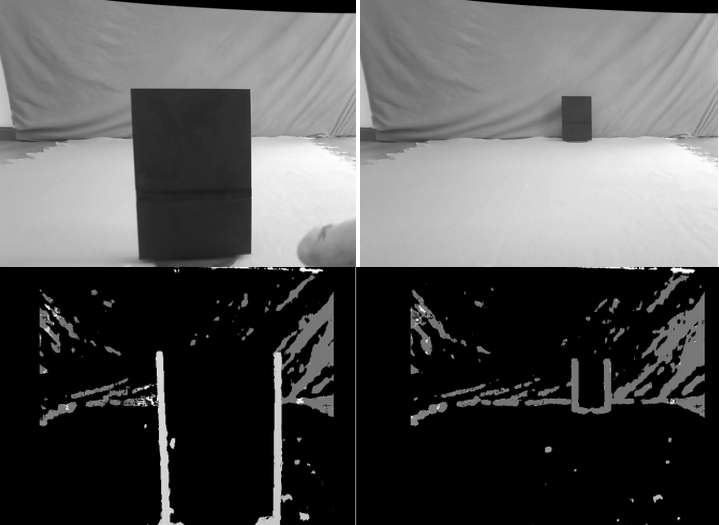
\includegraphics[width=1\textwidth]{f8.png}
  \caption{Imágenes originales y mapas de disparidad obtenidos con BM. Las imagenes izquierdas muestran el objeto a 0,5 m, y las imagenes derechas muestran el objeto a 1,83 m.}
\end{figure}

\begin{figure}[h!]

  \centering
    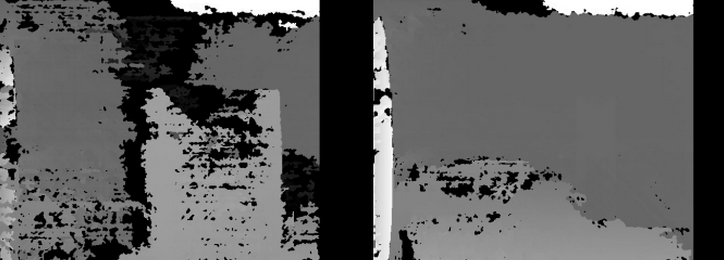
\includegraphics[width=1\textwidth]{f9.png}
  \caption{Imágenes originales y mapas de disparidad obtenidos con SGBM. Las imagenes izquierdas muestran el objeto a 0,5 m, y las imagenes derechas muestran el objeto a 1,72 m.}
\end{figure}

\begin{figure}[h!]

  \centering
    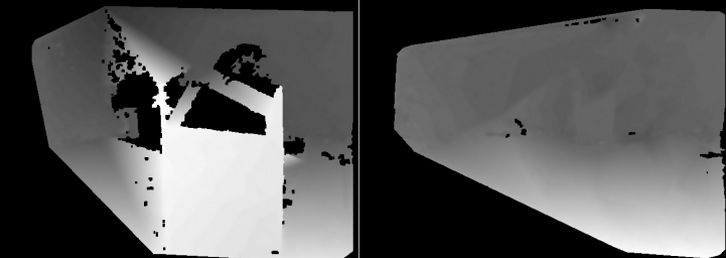
\includegraphics[width=1\textwidth]{f10.png}
  \caption{Imágenes originales y mapas de disparidad obtenidos con ELAS. Las imagenes izquierdas muestran el objeto a 0,5 m, y las imagenes derechas muestran el objeto a 1,83 m.}
\end{figure}

\subsubsection{Experimento 2}

En el anexo III se presenta una tabla con todas las mediciones de este experimento. Dada la gran cantidad de datos, aquí sólo se presenta una serie de gráficos y tablas para ayudar a interpretar estos datos.

En primer lugar se presenta y explica el cálculo de un factor que permite transformar los valores obtenidos por cada algoritmo a las mediciones de distancia (en cm).

Luego se presentan los valores obtenidos para los indicadores de precisión, recursos y densidad como fueron definidos previamente. En todos los casos se exponen la media, la desviación estándar y el percentil 95º de la muestra obtenida. En todos los indicadores se comparan los métodos de obtención del mapa de disparidad aunque en el caso de la precisión además se evaluan las distancias y los objetos utilizados.

\paragraph{Factor de escala}
\hfill \break
La distancia medida por cada método se calcula mediante la formula:

\[
	distancia = \frac{ factor_{m\acute{e}todo} }{ medici\acute{o}n }
\]

Dado que cada método tiene un factor desconocido de escala, se calculó la escala media y su error porcentual, mediante las siguientes fórmulas:

\[
	factor_{m\acute{e}todo} = \frac{1}{\#capturas} \sum_{captura} {distancia \times medici\acute{o}n}
\]

\[
	{\%\ error}_{m\acute{e}todo} = \frac{100 \  std_{captura}(distancia \times medici\acute{o}n)}{factor_{m\acute{e}todo}}
\]

Y los valores obtenidos son:

\begin{tabular}{ | l | c | c | c | }
	\hline
	& BM & SGBM & ELAS \\
	\hline
	factor & 25,965 & 418,429 & 414,265 \\
	\hline
	\% error & 1,031\% & 1,507\% & 1,520\% \\
	\hline
\end{tabular}

\paragraph{Errores}
\hfill \break
A continuación se muestra el histograma de todos los errores, y una tabla con la media, desviación estándar y percentil 95º de la muestra. A su vez, la \Figure{12} ilustra un histograma de todos los errores.

\begin{tabular}{ | c | c | }
	\hline
	& Error \\
	\hline
	Media & 0,002 m \\
	\hline
	Desviación estándar & 0,014 m \\
	\hline
	Percentil 95º & 0,028 m \\
	\hline
\end{tabular}

\begin{figure}[h!]

  \centering
    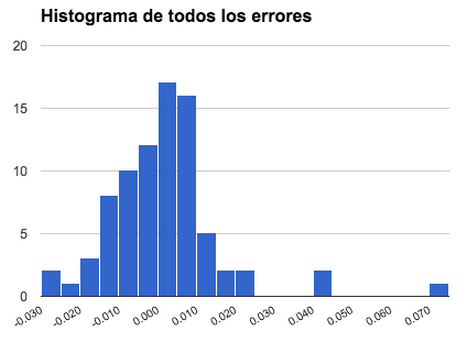
\includegraphics[width=0.7\textwidth]{f11.png}
  \caption{Histograma de los errores de todas las mediciones.}
\end{figure}

\paragraph{Errores por método}
\hfill \break
Es interesante ver los errores diferenciados por método de obtención de disparidades en conjunto con su histograma en la \Figure{13}

%% Dario Tabla 1

\begin{figure}[h!]

  \centering
    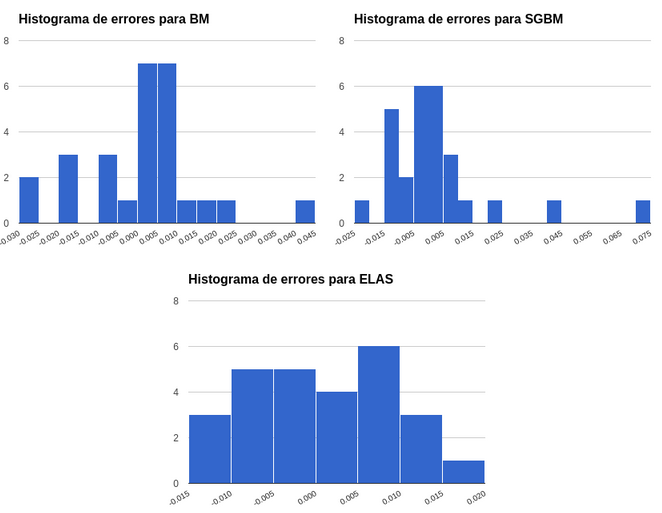
\includegraphics[width=1\textwidth]{f12.png}
  \caption{Histograma de los errores distinguidos por método.}
\end{figure}

\paragraph{Errores por objeto}
\hfill \break

Otro de los datos obtenidos en el Experimento 2 son los errores distinguidos por el objeto observado los cuales se presentan junto a sus histogramas en la \Figure{14}

%% Dario Tabla 2

\begin{figure}[h!]

  \centering
    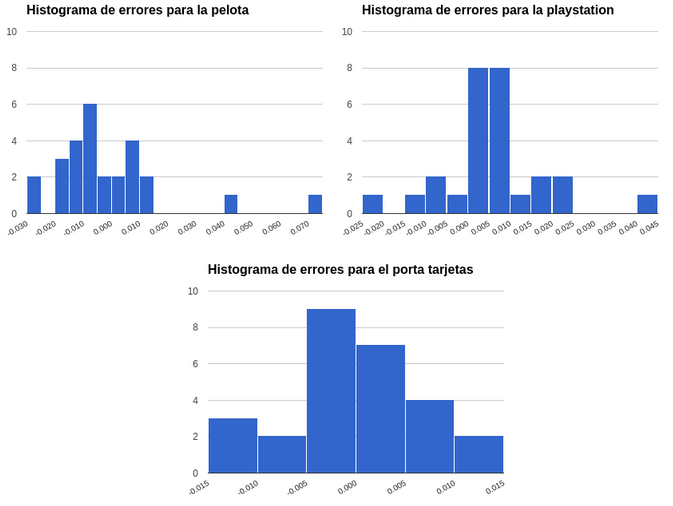
\includegraphics[width=1\textwidth]{f13.png}
  \caption{Histograma de los errores distinguidos por objeto.}
\end{figure}

\paragraph{Errores por distancia}
\hfill \break

Una última característica observable en cuanto a los errores que respectan a la precisión son los errores distinguidos por la distancia a medir. Este indicador también se presenta junto a sus histogramas en la \Figure{15}

%% Dario Tabla 3

\begin{figure}[h!]

  \centering
    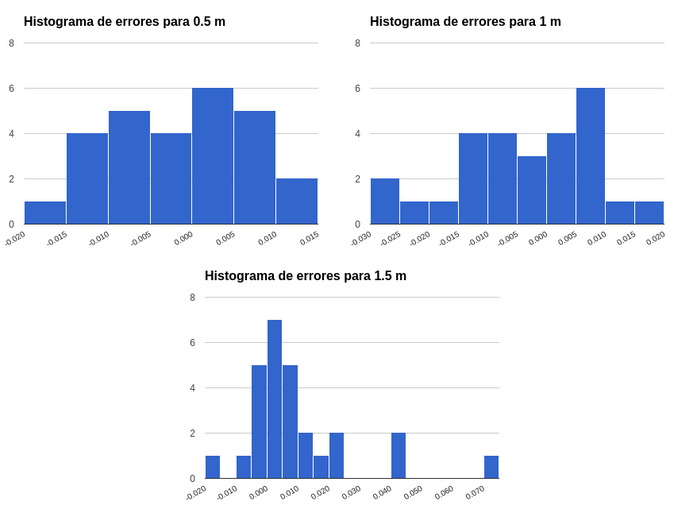
\includegraphics[width=1\textwidth]{f14.png}
  \caption{Histograma de los errores distinguidos por distancia a medir.}
\end{figure}

\paragraph{Tiempos por método}
\hfill \break

A la hora de medir los recursos, se presentan los tiempos de procesamiento de cada uno de los algoritmos. En la \Figure{16} se pueden ver sus histogramas.

%% Dario Tabla 4

\begin{figure}[h!]

  \centering
    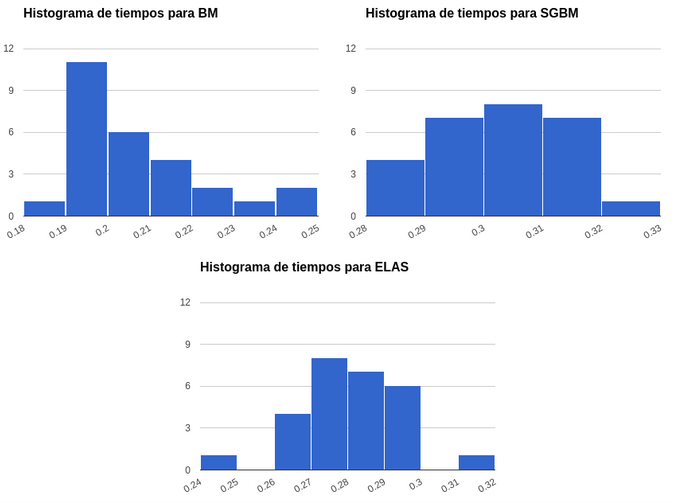
\includegraphics[width=1\textwidth]{f15.png}
  \caption{Histograma de los tiempos de procesamiento distinguidos por método.}
\end{figure}

\paragraph{Densidad por método}
\hfill \break

El último indicador del experimento 2 muestra la densidad obtenida para cada uno de los métodos. Para este indicador también se adjuntan sus histogramas en la \Figure{16}

%% Dario Tabla 5

\begin{figure}[h!]

  \centering
    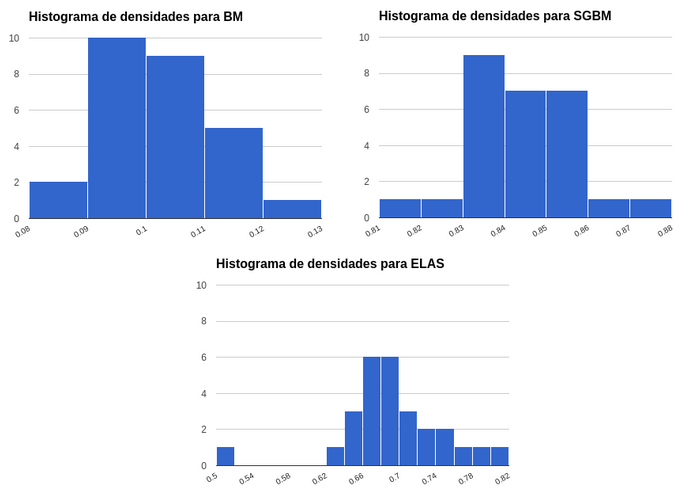
\includegraphics[width=1\textwidth]{f16.png}
  \caption{Histograma de las densidades obtenidas distinguidas por método.}
\end{figure}

\newpage

\section{Conclusiones y trabajo futuro}

Este último capítulo tiene como objetivo discutir las conclusiones obtenidas, basadas en los resultados de la experimentación, cerrando este informe con un análisis de la obtención de profundidades mediante cámaras estéreo.

En primer lugar, a diferencia de lo que se creía originalmente, durante la etapa de experimentación se encontró que el rango no sólo depende de la cámara, sino que también depende del método. Si bien todos los métodos proveen resultados precisos para distancias cortas (0,5 m), a distancias más grandes empiezan a aparecer algunas diferencias. Puntualmente, SGBM tiene un rango menor a los otros dos métodos.

En cuanto a la precisión de la cámara, los errores obtenidos tienen una media, un desvío estándar y un percentil que indican una alta precisión dentro del rango estudiado (con un error menor a 2 cm).

Al evaluar los errores encontrados en la precisión distinguidos por método se puede ver que ELAS es ligeramente superior al resto de los métodos. Si bien BM y SGBM comparten los órdenes de magnitud de estos errores, las muestras concretas indican una leve mejoría al obtener el mapa de disparidad utilizando BM.
Haciendo un análisis más profundo de estos errores podemos ver que los errores tanto en BM como en SGBM si bien se encuentran centradas en el 0 también presentan una tendencia a introducir casos espurios.
Si en vez de enfocarnos en los métodos nos enfocamos en los objetos medidos se puede ver que objetos pequeños y con esquinas definidas como el caso del porta tarjetas traen los mejores resultados. De forma opuesta, la pelota es el caso que más casos espurios y errores presenta. 
Como último dato al medir los errores de precisión aparece un pequeño análisis en cuanto a las distancias a medir. Al aumentar la distancia a medir aparecen más casos espurios aumentando el desvío estándar. De la misma manera, los errores comienzan a ser un poco más significativos.

La medición de los tiempos de procesamiento de los algoritmos muestran que todos comparten los órdenes de magnitud de este indicador. Sin embargo, en un análisis más profundo se puede ver que BM no solo tiene tiempos un poco más rápidos, sino que al analizar la curva que se forma se puede notar un detalle interesante. Mientras que SGBM y ELAS parecerían ser relativamente consistentes con sus tiempos, observamos que BM parece presentar una cola larga, indicando una predicción para este último algoritmo.

Por último, es importante hablar sobre las densidades que presenta cada uno de los algoritmos. Como es esperado, BM cuenta con una densidad notoriamente menor a los otros algoritmos. Esto es inherente al algoritmo ya que BM únicamente indica los bordes de los objetos encontrados. Si bien la diferencia entre SGBM y ELAS es menor, se puede ver que SGBM no solo posee una mayor densidad sino que también que su desvío estándar es menor que el de ELAS.

Como conclusiones finales, se puede ver que si bien es dependiente de la escena a analizar, las cámaras estéreo son un recurso accesible en el mércado que permite obtener resultados precisos en tiempo real. La aparición de cámaras portatiles en la actualidad es un indicio de que en caso de ser deseado, es posible extraer información de la profundidad de una escena de forma sencilla con diversas aplicaciones.
Aún más, al ser un procesamiento de imágenes, las cámaras estéreo no traen problemas de interferencia como si lo tendrían sensores de ultrasonido.

Si bien creemos que los resultados pueden ser mejorados mediante cámaras de mayor calidad, consideramos que la obtención de profundidades a través de cámaras estereo es un interesante recurso dado su accesibilidad.

\newpage

\section{Bibliografía}

\textbf{[CM03]} Coxeter, H. and Macdonald, S. "Projective geometry". Springer Science \& Business Media (2003).

\textbf{[EL03]} Elias, R. and Laganiere, R. "Projective geometry for three-dimensional computer vision". Paper in Viva Research Lab (2003).

\textbf{[B66]} Brown, D. "Decentering distortion of lenses". Photometric Engineering 32.3 (1966): 444-462.

\textbf{[Z00]} Zhang, Z. "A flexible new technique for camera calibration". Pattern Analysis and Machine Intelligence, IEEE Transactions on 22.11 (2000): 1330-1334.

\textbf{[Z04]} Zhang, Z. "Camera Calibration". Emerging topics in computer vision (2004): 4-43.

\textbf{[HS97]} Hartley, R. and Sturm, P. "Triangulation". Computer vision and image understanding 68.2 (1997): 146-157.

\textbf{[BT98]} Birchfield, S. and Tomasi, C. "A pixel dissimilarity measure that is insensitive to image sampling". Pattern Analysis and Machine Intelligence, IEEE Transactions on 20.4 (1998): 401-406.

\textbf{[T12]} Tippetts, B. "Real-Time Stereo Vision for Resource Limited Systems". (2012).

\textbf{[K98]} Konolige, K. "Small vision systems: Hardware and implementation". Robotics Research. Springer London (1998): 203-212.

\textbf{[GRU11]} Geiger, A., Roser, M. and Urtasun, R. "Efficient large-scale stereo matching". Computer Vision–ACCV 2010. Springer Berlin Heidelberg (2011): 25-38.

\textbf{[M93]} Matthies, L. "Stereo vision for planetary rovers: stochastic modeling to near realtime implementation". IJCV 8(1) (1993): 71-91.

\textbf{[BW93]} Bolles, R. and Woodfill, J. "Spatiotemporal consistency checking of passive range data". In International Symposium on Robotics Research, Vol. 32 (1993): 37.

\textbf{[H05]} Hirschmüller, H. "Accurate and efficient stereo processing by semi-global matching and mutual information". In Computer Vision and Pattern Recognition, 2005. CVPR 2005. IEEE Computer Society Conference on Vol. 2. IEEE (2005): 807-814.

\textbf{[EH08]} Ernst, I. and Hirschmüller, H. "Mutual information based semi-global stereo matching on the GPU". In Advances in Visual Computing. Springer Berlin Heidelberg. (2008): 228-239.

\textbf{[H08]} Hirschmüller, H. "Stereo processing by semiglobal matching and mutual information". Pattern Analysis and Machine Intelligence, IEEE Transactions on 30.2 (2008): 328-341.

\textbf{[SS02]} Scharstein, D. and Szeliski, R. (2002). "A taxonomy and evaluation of dense two-frame stereo correspondence algorithms". International journal of computer vision, 47(1-3), 7-42.

\begin{sloppypar}
\textbf{[OCV1]} http:\slash\slash docs.opencv.org\slash modules\slash calib3d\slash doc\slash camera\_calibration\_and\_3d\_reconstruction.html\#findchessboardcorners

\textbf{[OCV2]} http:\slash \slash docs.opencv.org\slash modules\slash imgproc\slash doc\slash feature\_detection.html\#cornersubpix

\textbf{[OCV3]} http:\slash \slash docs.opencv.org\slash modules\slash calib3d\slash doc\slash camera\_calibration\_and\_3d\_reconstruction.html\#calibratecamera

\textbf{[OCV4]} http:\slash \slash docs.opencv.org\slash modules\slash calib3d\slash doc\slash camera\_calibration\_and\_3d\_reconstruction.html\#stereocalibrate

\textbf{[OCV5]} http:\slash \slash docs.opencv.org\slash modules\slash calib3d\slash doc\slash camera\_calibration\_and\_3d\_reconstruction.html\#stereorectify

\textbf{[OCV6]} http:\slash \slash docs.opencv.org\slash modules\slash imgproc\slash doc\slash geometric\_transformations.html\#initundistortrectifymap

\textbf{[OCV7]} http:\slash \slash docs.opencv.org\slash modules\slash calib3d\slash doc\slash camera\_calibration\_and\_3d\_reconstruction.html\#stereobm

\textbf{[OCV8]} http:\slash \slash docs.opencv.org\slash modules\slash calib3d\slash doc\slash camera\_calibration\_and\_3d\_reconstruction.html\#stereosgbm
\end{sloppypar}

\textbf{[ELAS]} http://www.cvlibs.net/software/libelas/

\newpage

\section{Anexo I - Configuración de la Minoru}

La Webcam 3D Minoru es una cámara estereoscópica producida por Promotion and Display Technology of Salford, Greater Manchester lanzado en Enero del 2009.

La misma consiste en dos cámaras que se conectan a través de un puerto USB. Al poseer 2 cámaras puede reproducir imágenes 3D en donde cada cuadro puede variar entre 320x240 hasta 800x600 píxeles a una capacidad de 30 cuadros por segundo. Contiene 2 sensores VGA CMOS de 640x480 pixeles, lentes de ángulo ancho y un micrófono. Actualmente es obtenible en el mercado por 40 dólares.

Al obtener una cámara Minoru en su empaque original, la misma adjunta un CD que contiene un software utilizable en sistemas operativos de la familia Windows el cual permite ver imágenes 3D de forma rápida y sencilla.

Para el estudio presente se utilizó esta cámara en entornos UNIX encontrando ciertas dificultades en su uso, las cuales se encuentran aquí documentadas.

En primer lugar, acceder a más de una cámara mediante puertos USB en UNIX resulta en el siguiente error:

\begin{theorem}
libv4l2: error turning on stream: No space left on device VIDIOC\_STREAMON: No space left on device
\end{theorem}

Esto sucede ya que las cámaras intentan utilizar todo el ancho de banda disponible en el controlador USB, superando el ancho de banda disponible. Se puede resolver a través de los siguientes comandos.

\begin{theorem}
sudo rmmod uvcvideo
\end{theorem}

\begin{theorem}
sudo modprobe uvcvideo quirks=128
\end{theorem}

Estos comandos fuerzan a las cámaras a calcular el uso del ancho de banda en vez de utilizar el máximo, haciendo que el error desaparezca. Sin embargo, dada esta configuración, la resolución máxima que hemos podido obtener de las cámaras es de 640x480 píxeles a una capacidad de 23 cuadros por segundo. Cabe destacar que el número de quirks seleccionados no representa una cantidad, sino una máscara de bits que indica el modo en el que funcionara el módulo uvcvideo.
A pesar de los esfuerzos tratando de acceder a las cámaras mediante las funciones estándar en las librerías de OpenCV en OS X 10.10 (Yosemite), resulta imposible obtener información de ambas cámaras en simultáneo, generando un error en tiempo de ejecución. En Ubuntu 14.04 no se presenta este problema, pudiendo acceder a ambas cámaras como es esperado.

Por último, es importante mencionar que conectar una cámara Minoru en un puerto USB 3.0 trae diversos problemas, incluyendo la falta de capacidad para acceder a ambas cámaras en simultáneo y fallas en el driver del puerto.

\newpage

\section{Anexo II - Procedimiento en OpenCV}

Este anexo tiene como propósito documentar el procedimiento utilizado en el programa que obtiene el mapa de disparidad, utilizando funciones de OpenCV. Para esto se enumeran las funciones fundamentales especificando los parámetros de configuración. La implementación realizada fue hecha en C++.

De forma complementaria se utiliza la librería LibELAS.

Los criterios y parámetros utilizados son aquellos que de forma empírica han obtenido los mejores resultados.

Lo primero que se hace es la calibración de las cámaras. Para esto, primero, se utiliza la función \textbf{findChessboardCorners} \textbf{[OCV1]} la cual tiene como objetivo encontrar las esquinas internas de un tablero de ajedrez. Se utilizan los flags \textbf{CV\_CALIB\_CB\_ADAPTIVE\_THRESH} y \textbf{CV\_CALIB\_CB\_NORMALIZE\_IMAGE}. El primer flag indica que se usa una cota adaptativa para convertir la imagen a blanco y negro en vez de usar una cota fija. El segundo flag obliga a normalizar la imagen gamma antes de aplicar la cota antes mencionada.

\begin{sloppypar}
Para mejorar la precisión se utiliza función \textbf{cornerSubPix} \textbf{[OCV2]} utilizando como criterio \textbf{TermCriteria(CV\_TERMCRIT\_EPS | CV\_TERMCRIT\_ITER, 30, 0.1)}.
\textbf{CV\_TERMCRIT\_EPS} y \textbf{CV\_TERMCRIT\_ITER} le indica al algoritmo que la terminación del mismo será luego de que los resultados convergen a cierto valor o luego de determinada cantidad de iteraciones. Los siguientes parámetros indican los valores de terminación concretamente.
\end{sloppypar}

La calibración se realiza primero calibrando cada cámara por separado utilizando la función \textbf{calibrateCamera} \textbf{[OCV3]} y luego utilizando la función \textbf{stereoCalibrate} \textbf{[OCV4]}.

\begin{sloppypar}
Para \textbf{calibrateCamera} se utiliza como flag únicamente \textbf{CV\_CALIB\_FIX\_K3} lo cual indica que el parámetro de distorsión radial K3 (sección 2.2.3) no es modificado durante la optimización. Como criterio se utiliza \textbf{TermCriteria(CV\_TERMCRIT\_ITER | CV\_TERMCRIT\_EPS, INT\_MAX, DBL\_EPSILON)}.
\end{sloppypar}

En \textbf{stereoCalibrate} se utiliza el mismo criterio y los mismos flags que en \textbf{calibrateCamera} pero se agrega el flag \textbf{CV\_CALIB\_FIX\_INTRINSIC}. Esto indica que las matrices de las cámaras y los coeficientes de distorsión son fijados, de modo tal que sólo las matrices R, T, E, y F sean estimadas.

Luego se pasa a realizar la rectificación mediante la función \textbf{stereoRectify} \textbf{[OCV5]}. Se utilizan los parámetros por defecto de OpenCV (utilizando alpha como -1 y el flag \textbf{CV\_CALIB\_ZERO\_DISPARITY} el cual hace que los puntos principales de cada cámara tengan las mismas coordenadas en las vistas rectificadas).
Para finalizar la rectificación, se utiliza la función \textbf{initUndistortRectifyMap} \textbf{[OCV6]} la cual calcula los mapas de transformación para cada una de las imágenes.

Dependiendo del algoritmo elegido se utilizan las estructuras apropiadas, siendo estos StereoBM \textbf{[OCV7]}, StereoSGBM \textbf{[OCV8]} y ELAS \textbf{[ELAS]}.

Los parámetros utilizados para SGBM son los siguientes:

\begin{theorem}
sgbm.SADWindowSize = 5;
\end{theorem}

Esto indica el tamaño de las ventanas que serán comparadas entre ambas imágenes.

\begin{theorem}
sgbm.numberOfDisparities = 192;
\end{theorem}

Esto indica el rango de disparidades buscadas se encuentra en [minDisparity, minDisparity+numberOfDisparities].

\begin{theorem}
sgbm.preFilterCap = 4;
\end{theorem}

Se define una cota para los valores de salida a [-preFilterCap, preFilterCap]

\begin{theorem}
sgbm.minDisparity = -64;
\end{theorem}

Se define el menor valor de disparidad que es tomado en cuenta.

\begin{theorem}
sgbm.uniquenessRatio = 1;
\end{theorem}

Este valor define otro filtro para los valores aceptados por las disparidades.

\begin{theorem}
sgbm.speckleWindowSize = 150;
\end{theorem}

Este valor es el tamaño máximo de regiones de disparidad para considerar (e invalidar) ruido Speckle.

\begin{theorem}
sgbm.speckleRange = 2;
\end{theorem}

Esto define la máxima variación de las disparidades entre cada componente conectado.

\begin{theorem}
sgbm.disp12MaxDiff = 10;
\end{theorem}

Bajo este valor se marca la diferencia permitida (en cantidad de píxeles) al hacer el chequeo izquierdo-derecho de disparidad.

\begin{theorem}
sgbm.fullDP = false;
\end{theorem}

Al indicar este parámetro como falso, se utiliza una versión menos optimizada del algoritmo, mucho más económico en el uso de la memoria.

\begin{theorem}
sgbm.P1 = 600;
\end{theorem}
\begin{theorem}
sgbm.P2 = 2400;
\end{theorem}

Estos parámetros indican la suavidad de la disparidad. Cuanto más grandes son estos valores, mejores son los resultados. Ambos valores aplican castigos a la diferencia de disparidad entre píxeles vecinos.


Los parámetros utilizados para BM son los siguientes:

\begin{theorem}
sbm.SADWindowSize = 9;
\end{theorem}
\begin{theorem}
sbm.speckleWindowSize = 0;
\end{theorem}
\begin{theorem}
sbm.speckleRange = 8;
\end{theorem}
\begin{theorem}
sbm.disp12MaxDiff = 1;
\end{theorem}
\begin{theorem}
sbm.numberOfDisparities = 112;
\end{theorem}
\begin{theorem}
sbm.minDisparity = -39;
\end{theorem}
\begin{theorem}
sbm.preFilterCap = 61;
\end{theorem}
\begin{theorem}
sbm.uniquenessRatio = 0;
\end{theorem}

Estos primeros 8 parámetros indican lo mismo que en SGBM.

\begin{theorem}
sbm.preFilterSize = 5;
\end{theorem}

Se indica el tamaño de la ventana del filtro previo que se aplica.

\begin{theorem}
sbm.textureThreshold = 507;
\end{theorem}

Se calcula la disparidad en donde la textura supera la cota indicada.

\newpage

\section{Anexo III: Resultados del Experimento 2}

A continuación se detalla la tabla con los resultados del Experimento 2.

%% Dario Tabla 6

\end{document}
